\documentclass[11pt,a4paper]{article}
\usepackage[utf8]{inputenc}
\usepackage[french]{babel}
\usepackage[T1]{fontenc}

\usepackage{amsmath}
\usepackage{amsfonts}
\usepackage{amssymb}

\newcommand{\NomAuteur}{Fabrice BOISSIER}
\newcommand{\TitreMatiere}{Algo et Structure de Données 1}
\newcommand{\NomUniv}{EPITA - Bachelor Cyber Sécurité}
\newcommand{\NiveauUniv}{CYBER1}
\newcommand{\NumGroupe}{CYBER1}
\newcommand{\AnneeUniv}{2022-2023}
\newcommand{\DateExam}{janvier 2023}
\newcommand{\TypeExam}{Partiel (Sujet 2)}
\newcommand{\TitreExam}{\TitreMatiere}
\newcommand{\DureeExam}{2h00}
\newcommand{\MyWaterMark}{\AnneeUniv} % Watermark de protection

% Ajout de mes classes & definitions
\usepackage{MetalExam} % Appelle un .sty

% "Tableau" et pas "Table"
\addto\captionsfrench{\def\tablename{Tableau}}

%%%%%%%%%%%%%%%%%%%%%%%
%Header
%%%%%%%%%%%%%%%%%%%%%%%
\lhead{\TypeExam}							%Gauche Haut
\chead{\NomUniv}							%Centre Haut
\rhead{\NumGroupe}							%Droite Haut
\lfoot{\DateExam}							%Gauche Bas
\cfoot{\thepage{} / \pageref*{LastPage}}	%Centre Bas
\rfoot{\texttt{\TitreMatiere}}				%Droite Bas

%%%%%

\usepackage{tabularx}

\newlength{\LabelWidth}%
%\setlength{\LabelWidth}{1.3in}%
\setlength{\LabelWidth}{1cm}%
%\settowidth{\LabelWidth}{Employee E-mail:}%  Specify the widest text here.

% Optional first parameter here specifies the alignment of
% the text within the \makebox.  Default is [l] for left
% alignment. Other options are [r] and [c] for right and center
\newcommand*{\AdjustSize}[2][l]{\makebox[\LabelWidth][#1]{#2}}%


\definecolor{mGreen}{rgb}{0,0.6,0}
\definecolor{mGray}{rgb}{0.5,0.5,0.5}
\definecolor{mPurple}{rgb}{0.58,0,0.82}
\definecolor{backgroundColour}{rgb}{0.95,0.95,0.92}

\lstdefinestyle{CStyle}{
    backgroundcolor=\color{backgroundColour},
    commentstyle=\color{mGreen},
    keywordstyle=\color{magenta},
    numberstyle=\tiny\color{mGray},
    stringstyle=\color{mPurple},
    basicstyle=\footnotesize,
    breakatwhitespace=false,
    breaklines=true,
    captionpos=b,
    keepspaces=true,
    numbers=left,
    numbersep=5pt,
    showspaces=false,
    showstringspaces=false,
    showtabs=false,
    tabsize=2,
    language=C
}


\hyphenation{op-tical net-works SIGKILL}


\begin{document}

%\MakeExamTitleDuree     % Pour afficher la duree
\MakeExamTitle                   % Ne pas afficher la duree

%% \MakeStudentName    %% A reutiliser sur chaque nouvelle page

\bigskip
\bigskip

Vous devez respecter les consignes suivantes, sous peine de 0 :

\begin{itemize}
\item Lisez le sujet en entier avec attention
\item Répondez sur le sujet
\item Ne détachez pas les agrafes du sujet
\item \'Ecrivez lisiblement vos réponses (si nécessaire en majuscules)
\item Vous devez écrire dans le langage algorithmique ou en C (donc pas de Python ou autre)
\item Ne trichez pas
\end{itemize}

\bigskip

%%%%%%%%%%%%%%%%% CENTRAGE
\vfillFirst

Dans cet examen, vous allez implémentez avec précisions quelques opérations basiques d'utilisation d'une liste (taille de la liste, récupération du premier élément, récupération du dernier élément, test si la liste est vide, ajout d'un élément à un emplacement précis en poussant les éléments suivants, suppression d'un élément suivi d'une copie des éléments suivants, vider la liste), et vous utiliserez ces opérations pour implémenter une pile et une file.

\hspace{2cm}

% Questions cours
\section{Questions (6 points)}

\bigskip

\begin{figure}[ht!]
\centering
\centerline{  %%% CENTRAGE HORIZONTAL
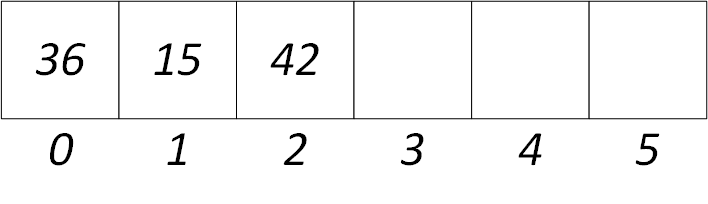
\includegraphics[height=3cm]{img/Liste_t_1.png}
%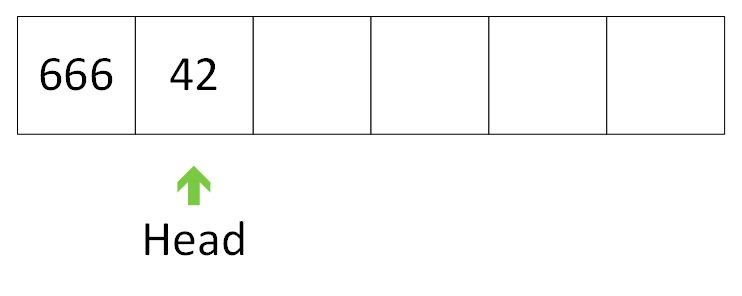
\includegraphics[scale=1,left]{img/2_elts.png}
}
%\caption{File A}
%\label{figure:1-S1-ModeleWI}
\end{figure}


\bigskip

\subsection{(1 point) Donnez les caractéristiques de cette liste : }

\bigskip

\begin{table}[h!]
  \centering
  \begin{minipage}{0.25\textwidth}
    \centering
Taille de la liste :

\medskip

\begin{tabular}{ | m{2.5cm} | }
\hline
 \\ \\ \\ \\ \\ \\
\hline
\end{tabular}

  \end{minipage}
  \hfillx
  \begin{minipage}{0.25\textwidth}
    \centering
Taille maximale de la liste :

\medskip

\begin{tabular}{ | m{2.5cm} | }
\hline
 \\ \\ \\ \\ \\ \\
\hline
\end{tabular}

  \end{minipage}
  \hfillx
  \begin{minipage}{0.25\textwidth}
    \centering
Tête de la liste :

\medskip

\begin{tabular}{ | m{2.5cm} | }
\hline
 \\ \\ \\ \\ \\ \\
\hline
\end{tabular}

  \end{minipage}
  \hfillx
  \begin{minipage}{0.25\textwidth}
    \centering
Queue de la liste :

\medskip

\begin{tabular}{ | m{2.5cm} | }
\hline
 \\ \\ \\ \\ \\ \\
\hline
\end{tabular}

  \end{minipage}
\end{table}

\bigskip

\vfillLast
%%%%%%%%%%%%%%%%% CENTRAGE

\newpage

\subsection{(2,5 points) Indiquez l'état de la liste après chacune de ces opérations, puis précisez à quelle structure de données ce comportement correspond. }

%\bigskip

\begin{figure}[ht!]
\centering
\centerline{  %%% CENTRAGE HORIZONTAL
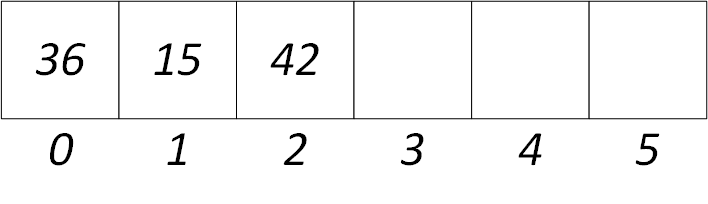
\includegraphics[height=2cm]{img/Liste_t_1.png}
%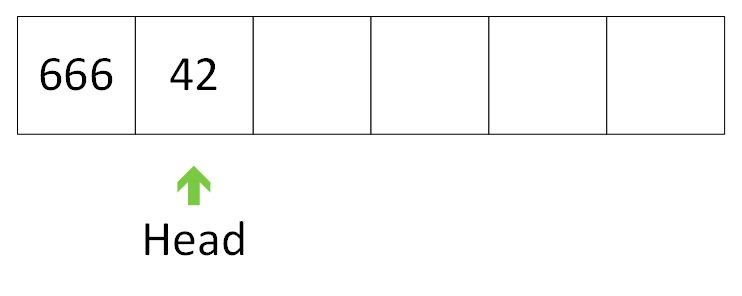
\includegraphics[scale=1,left]{img/2_elts.png}
}
\end{figure}

\begin{center}

\texttt{Ajout de 55 en première position en décalant les valeurs vers la fin}

\begin{figure}[ht!]
\centering
\centerline{  %%% CENTRAGE HORIZONTAL
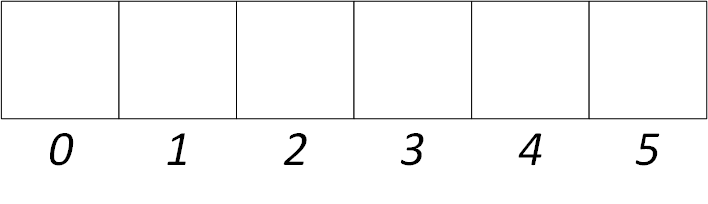
\includegraphics[height=2cm]{img/Liste_t_vide.png}
%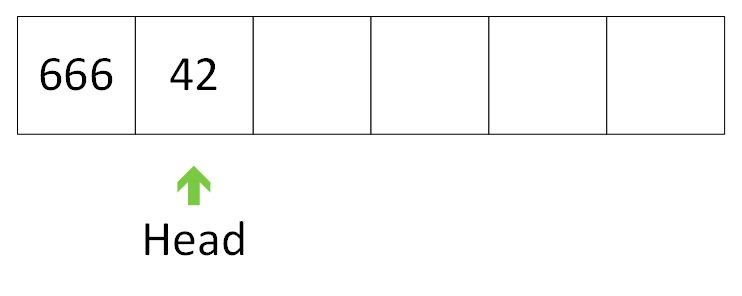
\includegraphics[scale=1,left]{img/2_elts.png}
}
\end{figure}


\texttt{Ajout de 14 en première position en décalant les valeurs vers la fin}

\begin{figure}[ht!]
\centering
\centerline{  %%% CENTRAGE HORIZONTAL
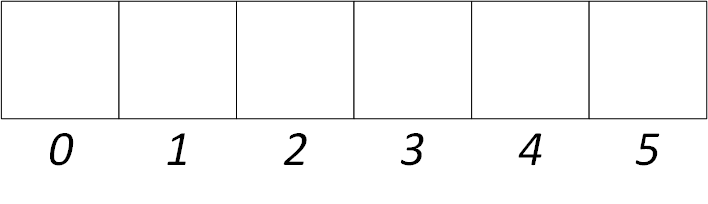
\includegraphics[height=2cm]{img/Liste_t_vide.png}
%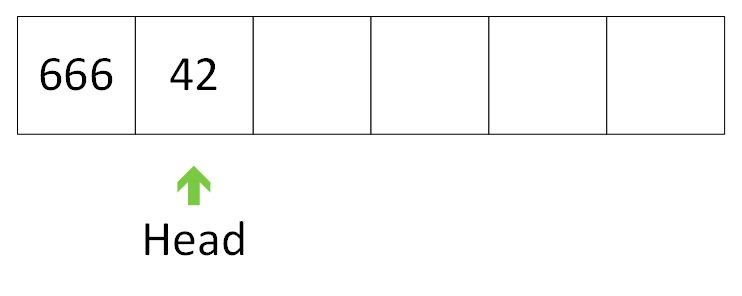
\includegraphics[scale=1,left]{img/2_elts.png}
}
\end{figure}


\texttt{Ajout de 21 en première position en décalant les valeurs vers la fin}

\begin{figure}[ht!]
\centering
\centerline{  %%% CENTRAGE HORIZONTAL
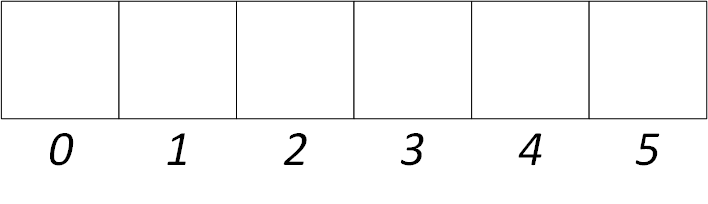
\includegraphics[height=2cm]{img/Liste_t_vide.png}
%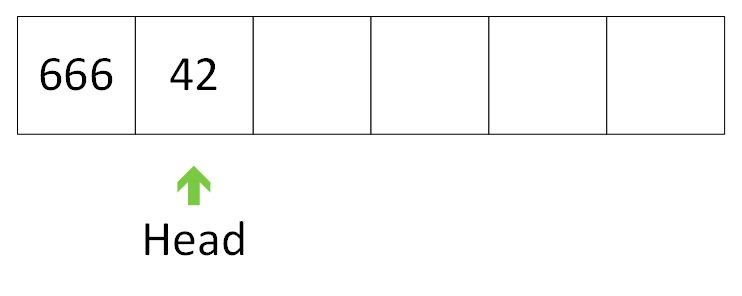
\includegraphics[scale=1,left]{img/2_elts.png}
}
\end{figure}


\texttt{Suppression de la première position en décalant les valeurs vers le début}

\begin{figure}[ht!]
\centering
\centerline{  %%% CENTRAGE HORIZONTAL
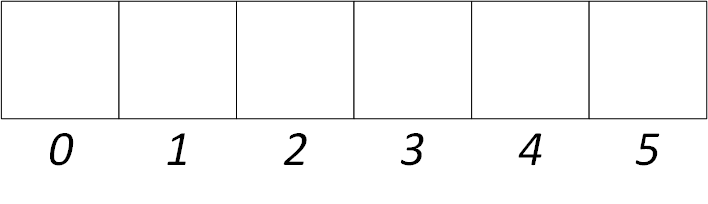
\includegraphics[height=2cm]{img/Liste_t_vide.png}
%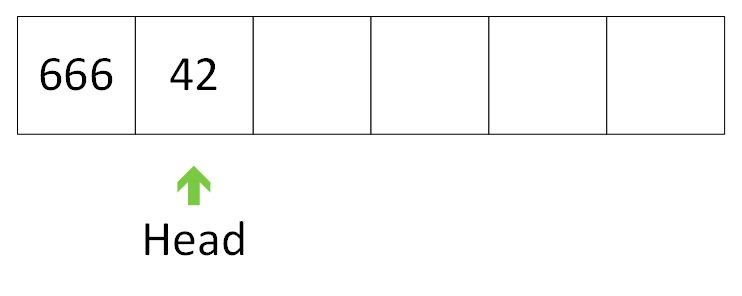
\includegraphics[scale=1,left]{img/2_elts.png}
}
\end{figure}


\texttt{Suppression de la première position en décalant les valeurs vers le début}

\begin{figure}[ht!]
\centering
\centerline{  %%% CENTRAGE HORIZONTAL
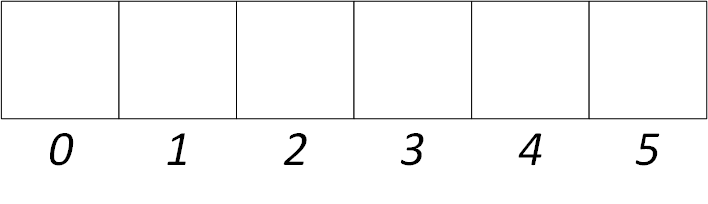
\includegraphics[height=2cm]{img/Liste_t_vide.png}
%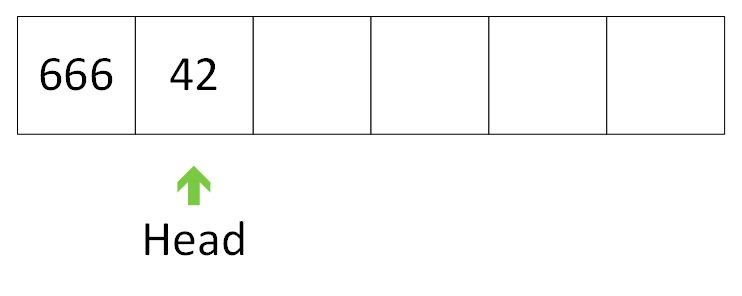
\includegraphics[scale=1,left]{img/2_elts.png}
}
\end{figure}


\texttt{Suppression de la première position en décalant les valeurs vers le début}

\begin{figure}[ht!]
\centering
\centerline{  %%% CENTRAGE HORIZONTAL
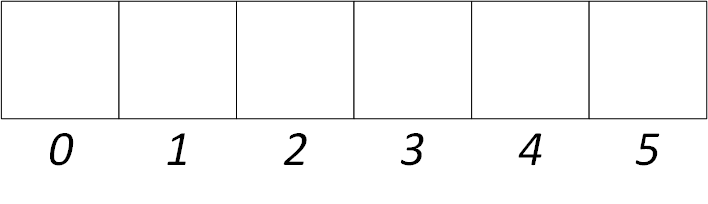
\includegraphics[height=2cm]{img/Liste_t_vide.png}
%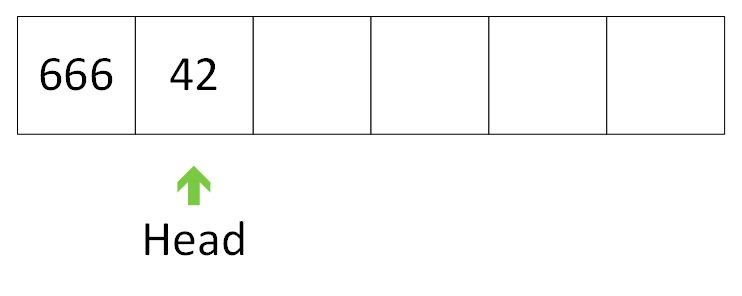
\includegraphics[scale=1,left]{img/2_elts.png}
}
\end{figure}

%\bigskip

\end{center}

Structure de données imitée :



\newpage

\subsection{(2,5 points) Indiquez l'état de la liste après chacune de ces opérations, puis précisez à quelle structure de données ce comportement correspond. }

%\bigskip

\begin{figure}[ht!]
\centering
\centerline{  %%% CENTRAGE HORIZONTAL
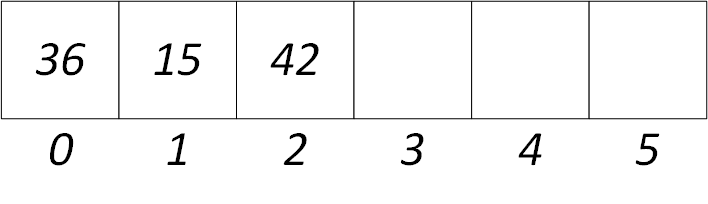
\includegraphics[height=2cm]{img/Liste_t_1.png}
%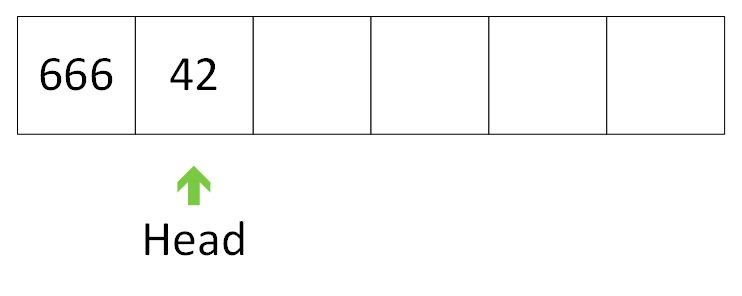
\includegraphics[scale=1,left]{img/2_elts.png}
}
\end{figure}

\begin{center}

\texttt{Ajout de 55 en \textit{dernière} position}

\begin{figure}[ht!]
\centering
\centerline{  %%% CENTRAGE HORIZONTAL
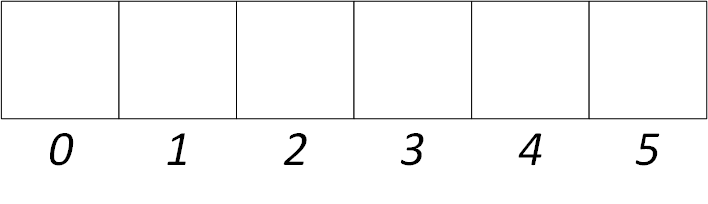
\includegraphics[height=2cm]{img/Liste_t_vide.png}
%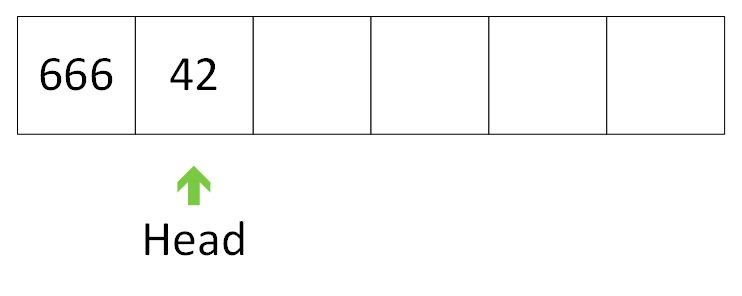
\includegraphics[scale=1,left]{img/2_elts.png}
}
\end{figure}


\texttt{Ajout de 14 en \textit{dernière} position}

\begin{figure}[ht!]
\centering
\centerline{  %%% CENTRAGE HORIZONTAL
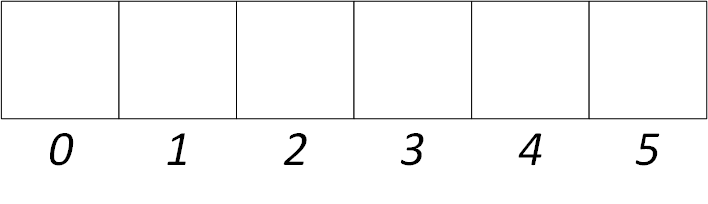
\includegraphics[height=2cm]{img/Liste_t_vide.png}
%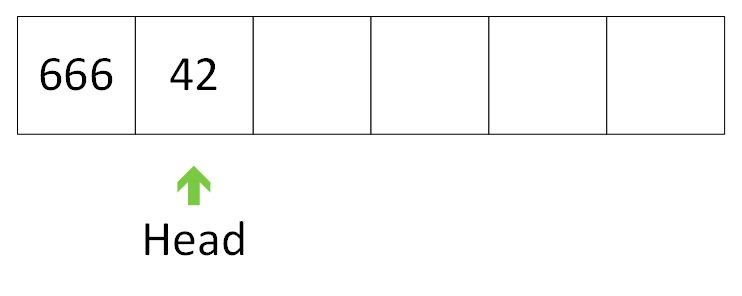
\includegraphics[scale=1,left]{img/2_elts.png}
}
\end{figure}


\texttt{Ajout de 21 en \textit{dernière} position}

\begin{figure}[ht!]
\centering
\centerline{  %%% CENTRAGE HORIZONTAL
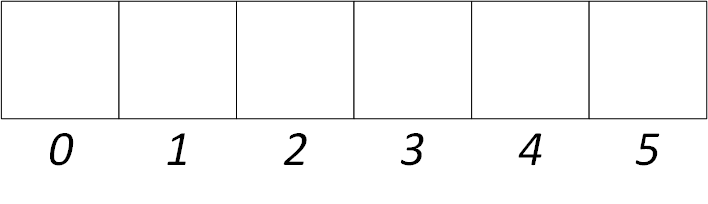
\includegraphics[height=2cm]{img/Liste_t_vide.png}
%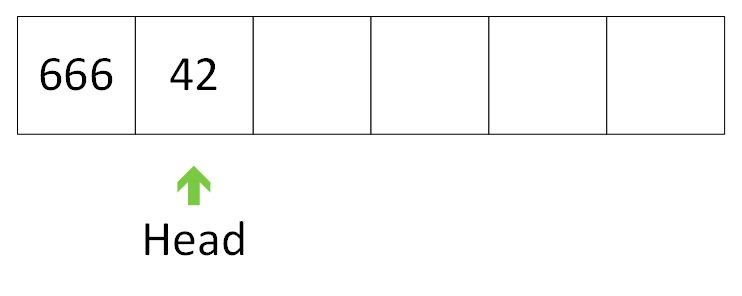
\includegraphics[scale=1,left]{img/2_elts.png}
}
\end{figure}


\texttt{Suppression de la première position en décalant les valeurs vers le début}

\begin{figure}[ht!]
\centering
\centerline{  %%% CENTRAGE HORIZONTAL
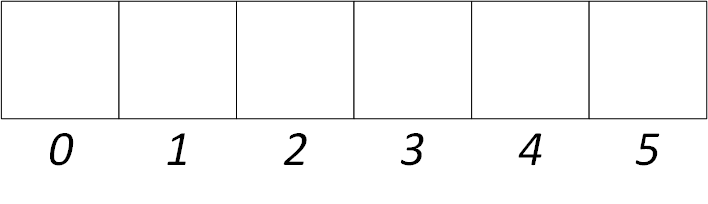
\includegraphics[height=2cm]{img/Liste_t_vide.png}
%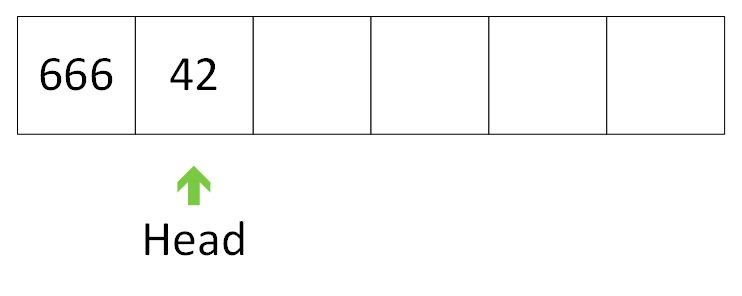
\includegraphics[scale=1,left]{img/2_elts.png}
}
\end{figure}


\texttt{Suppression de la première position en décalant les valeurs vers le début}

\begin{figure}[ht!]
\centering
\centerline{  %%% CENTRAGE HORIZONTAL
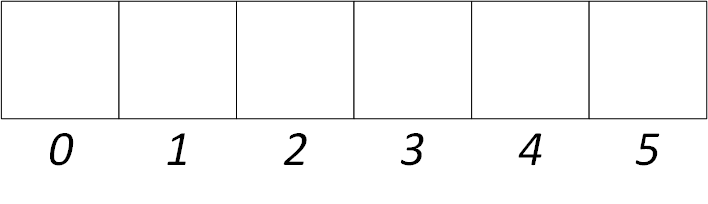
\includegraphics[height=2cm]{img/Liste_t_vide.png}
%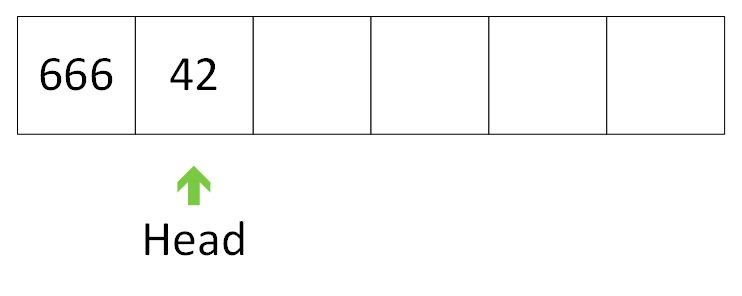
\includegraphics[scale=1,left]{img/2_elts.png}
}
\end{figure}


\texttt{Suppression de la première position en décalant les valeurs vers le début}

\begin{figure}[ht!]
\centering
\centerline{  %%% CENTRAGE HORIZONTAL
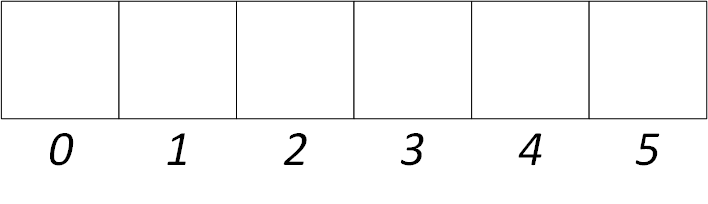
\includegraphics[height=2cm]{img/Liste_t_vide.png}
%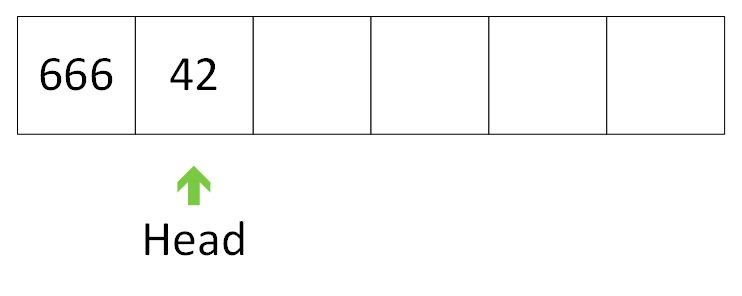
\includegraphics[scale=1,left]{img/2_elts.png}
}
\end{figure}

%\bigskip

\end{center}

Structure de données imitée :

\bigskip



\newpage

%
\section{Algorithmes (14 points)}

Le but de l'implémentation est de réutiliser les fonctions que vous écrirez.
Si vous ne savez pas implémenter une des fonctions, vous pouvez tout de même l'utiliser dans les exercices suivants.

%%%%%%%%%%%%%%%%% CENTRAGE
\vfillFirst

\subsection*{A - Liste à tableau}

\subsection{(1 point) \'Ecrivez une structure de données \og \textit{my\_list\_t} \fg{} pouvant servir de liste contenant des éléments étant des entiers positifs. Cette liste doit être stockée dans un tableau (et non pas une chaîne de pointeurs). }

\bigskip

\begin{center}
\GrilleReponseN{7}
\end{center}

\bigskip

\subsection{(2 points) \'Ecrivez l'implémentation des fonctions suivantes : }

\begin{itemize}
\item \textit{length\_list} : renvoie la taille de la liste, c'est-à-dire le nombre d'éléments contenus
\item \textit{get\_first\_elt} : renvoie le premier élément de la liste
\item \textit{get\_last\_elt} : renvoie le dernier élément de la liste
\item \textit{list\_is\_empty} : renvoie \textit{vrai} si la liste est vide, sinon \textit{faux}
\item \textit{list\_is\_full} : renvoie \textit{vrai} si la liste est pleine, sinon \textit{faux}
\end{itemize}

\bigskip

\texttt{int length\_list(my\_list\_t *liste)}

\begin{center}
\GrilleReponseN{7}
\end{center}

%\medskip

\vfillLast
%%%%%%%%%%%%%%%%% CENTRAGE

\newpage

%%%%%%%%%%%%%%%%% CENTRAGE
\vfillFirst

\texttt{int get\_first\_elt(my\_list\_t *liste)}

\begin{center}
\GrilleReponseN{5}
\end{center}

\medskip

\texttt{int get\_last\_elt(my\_list\_t *liste)}

\begin{center}
\GrilleReponseN{5}
\end{center}

\medskip

\texttt{bool list\_is\_empty(my\_list\_t *liste)}

\begin{center}
\GrilleReponseN{5}
\end{center}

\medskip

\texttt{bool list\_is\_full(my\_list\_t *liste)}

\begin{center}
\GrilleReponseN{5}
\end{center}

\vfillLast
%%%%%%%%%%%%%%%%% CENTRAGE

\newpage

\subsection{(3 points) \'Ecrivez une fonction \og \textit{add\_elt\_at\_pos} \fg{} qui ajoute un élément \textit{elt} à la position \textit{pos} dans la liste \textit{liste}, puis renvoie \textit{vrai}. Si la position est déjà occupée, vous décalerez son contenu et celui des cellules suivantes d'un cran vers la fin. Si la liste est pleine ou si la position n'existe pas, vous renverrez \texttt{faux} sans rien faire. La position 0 est considérée comme la première position de la liste. }

\bigskip

\texttt{bool add\_elt\_at\_pos(my\_list\_t *liste, int elt, int pos)}

\begin{center}
\GrilleReponseN{21}
\end{center}

\newpage

\subsection{(3 points) \'Ecrivez une fonction \og \textit{del\_elt\_at\_pos} \fg{} qui supprime l'élément de la position \textit{pos} dans la liste \textit{liste}, puis renvoie \textit{vrai}. Vous décalerez les cellules suivantes d'un cran vers le début. Si la liste est vide ou si la position n'existe pas, vous renverrez \texttt{faux} sans rien faire. La position 0 est considérée comme la première position de la liste. }

\bigskip

\texttt{bool del\_elt\_at\_pos(my\_list\_t *liste, int pos)}

\begin{center}
\GrilleReponseN{21}
\end{center}

\newpage

\subsection{(1 point) \'Ecrivez une fonction \og \textit{remove\_list} \fg{} qui vide la liste \textit{liste} en supprimant tous les éléments contenus dedans. }

\bigskip

\texttt{void remove\_list(my\_list\_t *liste)}

\begin{center}
\GrilleReponseN{9}
\end{center}


%\newpage


\subsection*{B - Pile et File avec liste à tableau}

Vous allez maintenant utiliser les fonctions que vous venez d'écrire pour implémenter des piles et des files.
Vous devez réutiliser les fonctions existantes (non pas en les réécrivant, mais en les appelant).
N'hésitez pas à relire vos réponses de la partie \textit{Questions} pour vous aider.

\subsection{(1 point) \'Ecrivez une fonction \og \textit{push} \fg{} pouvant servir à empiler un élément dans une liste. }

\bigskip

\begin{center}
\GrilleReponseN{9}
\end{center}

\newpage

\subsection{(1 point) \'Ecrivez une fonction \og \textit{pop} \fg{} pouvant servir à dépiler un élément depuis une liste. }

\bigskip

\begin{center}
\GrilleReponseN{10}
\end{center}

\bigskip



%\newpage

\subsection{(1 point) \'Ecrivez une fonction \og \textit{enqueue} \fg{} pouvant servir à enfiler un élément dans une liste. }

\bigskip

\begin{center}
\GrilleReponseN{10}
\end{center}

%\newpage

\subsection{(1 point) \'Ecrivez une fonction \og \textit{dequeue} \fg{} pouvant servir à défiler un élément depuis une liste. }

\bigskip

\begin{center}
\GrilleReponseN{10}
\end{center}

\bigskip

\end{document}
